\documentclass[unnumsec,webpdf,contemporary,large]{oup-authoring-template}

\graphicspath{{figures/}}
\usepackage{booktabs}
\usepackage{array}
\usepackage{setspace}
\usepackage{lineno}
\usepackage{placeins}
\usepackage{float}
\usepackage{xcolor}
\setcitestyle{numbers,super,sort&compress}

\newcommand{\visiblealt}[1]{\figalttext{Alt text: #1}\par\smallskip\noindent{\small\textbf{Alt text:} #1}\par}
\usepackage{soul}
\newcommand{\td}[1]{\sethlcolor{pink}\hl{[Ting: #1]}}
\newcommand{\hy}[1]{\sethlcolor{yellow}\hl{[HY: #1]}}
\begin{document}
\onehalfspacing % TEST: was \doublespacing
\linenumbers

\journaltitle{Journal of the American Medical Informatics Association}
\copyrightyear{2026}
\pubyear{2026}
\appnotes{Research and Applications}

\title[Stigmatizing language by section audience]{Comparing Stigmatizing Language Across Clinician-Facing and Patient-Facing within Clinical notes}
\author[1,$\ast$]{Author names and degrees required}
\address[1]{Author input required: department, institution, city, and country for every author.}
\corresp[$\ast$]{Author input required: corresponding author postal address, email, and telephone. Main text word count: 3,872.}

\abstract{\textbf{Objective:} Stigmatizing language in clinical notes can influence clinicians’ judgements and treatment decisions, with potential consequences for patient outcomes. Its occurrence may also vary according to note function and intended audience. We aimed to quantify differences in stigmatizing language between clinician-facing and patient-facing note functions and to examine how these differences varied across patient cohorts.\\
\textbf{Materials and Methods:} We analyzed 259,207 notes from MIMIC-IV-Note, extracting the clinician-facing Brief Hospital Course (BHC) and History of Present Illness (HPI) sections and the patient-facing Discharge Instructions (DI) section. A GatorTron-based language model as classifier identified stigmatizing language. Poisson generalized model compared rates of stigmatizing language across note functions and examined whether these differences varied across patient cohorts.\\
\textbf{Results:} The GatorTron-based classifier achieved a test macro-F1 score of 0.928. Rates of stigmatizing language were 8.21 times higher in BHC than in DI and 7.21 times higher in HPI than in DI. Patient cohorts with the highest rates of stigmatizing language in patient-facing instructions were not necessarily those with the largest clinician-facing versus patient-facing differences.\\
\hy{TODO}
\textbf{Discussion:} Stigmatizing language was strongly patterned by section audience. Whole-note estimates combine clinician-facing narrative with patient-facing instructions, obscuring where the language appears and how patient-group patterns differ across these settings.\\
\textbf{Conclusion:} Section-aware measurement distinguishes stigmatizing language in clinician-facing documentation from that in patient-facing instructions and identifies where audience-specific documentation review could focus.}

\keywords{electronic health records, social stigma, natural language processing, clinical documentation, health equity}

\maketitle

\boxedtext{Key Messages}{
\begin{spacing}{1.0}
\small
\noindent Stigmatizing language is well documented in clinician-facing clinical notes, but the extent to which its use changes when documentation is written for patients remains unclear. Across 259,207 note pairs, stigmatizing language was 8.21 times as frequent in clinician-facing notes as in patient-facing discharge notes for BHC, and 7.21 times as frequent for HPI.\par\smallskip
\noindent \hy{TODO: The disparity results, still running}
\end{spacing}}
\td{I am not familiar with the journal, so I am not sure what its general writing style is. To me, the Materials and Methods section reads with a bit too much detail, and the names of the methods may not be the most important part. Instead, the key idea should be emphasized: you used machine learning methods to develop the stigmatizing language recognizer and you compared the recognition rate or sth similar, between the two sets of notes. It would also be helpful to clarify that you further compare the ratio or sth across different social-demographic/disease groups.}
\td{results part are a bit hard to follow. For example, bhc-di rate ratio and adjusted rate ratios, what are they and what do they imply? discussion could be focusing more on what might lead to this? }
\section{Background and Significance}
%% why stigma is important
Stigma occurs when labeling and stereotyping co-occur with separation, status loss, and discrimination in a context of unequal power.\cite{link2001} It contributes to population health inequalities by shaping access to material, social, and healthcare resources through structural, interpersonal, and psychological pathways.\cite{hatzenbuehler2013} Clinical documentation can instantiate these pathways: stigmatizing descriptions entered into the record persist, travel to subsequent clinicians, and have been shown to worsen provider attitudes and pain-management decisions.\cite{goddu2018} These effects extend beyond individual encounters. Once documentation recorded, stigmatizing language becomes part of the patient's longitudinal record, where it can shape how subsequent clinicians interpret symptoms, assess credibility, and allocate treatment.\cite{goddu2018,park2021} Patients who read their own notes may also encounter this language directly, potentially undermining trust and engagement with the healthcare system.\cite{leveille2020notes} Clinical documentation thus functions not only as a record of care but as a channel through which stigma is reproduced across providers and transmitted to patients.
 
%% stigma can be different ... previous ...
Stigmatizing language in clinical records takes multiple forms, including expressions of doubt and disapproval, negative stereotyping, difficult-patient framing, and assertions of clinician authority.\cite{park2021,mcarthur2026} Its prevalence also varies across patient populations: studies have found higher rates of stigmatizing language in notes for patients with substance use disorders, chronic pain, and disability compared with other conditions, as well as disparities by recorded race and ethnicity.\cite{himmelstein2022, sun2022} However, clinical documentation is not a uniform communicative space. Discharge summaries, for example, contain sections written primarily for clinicians alongside sections written directly for patients.\cite{li2026readability} Existing studies have largely examined clinician-facing narratives without distinguishing whether their findings extend to patient-facing text.

%% introducing section diff
This distinction matters because clinical documentation serves different audiences and functions.\cite{li2026readability} Within a discharge summary, the Brief Hospital Course (BHC) and History of Present Illness (HPI) describe the patient's clinical history and hospital encounter primarily for other clinicians, whereas the Discharge Instructions (DI) communicate information about follow-up care, medications, precautions, and self-care to patients.\cite{xu2024dischargeme,li2026readability} Stigmatizing language in clinician-facing sections may frame subsequent clinical interpretation and influence treatment decisions.\cite{goddu2018} In DI, such language becomes part of direct patient-facing communication, where patients may encounter wording they perceive as judgmental.\cite{leveille2020notes,li2026readability} To our knowledge, prior work has not compared patient-facing DI with clinician-facing sections from the same discharge summary. It therefore remains unclear whether stigmatizing language persists, decreases, or changes when clinicians write directly for patients.

%% intro nlp model used in stigma detection
Natural language processing has made it possible to identify stigmatizing language at scale. \cite{harrigian2023,xue2026,walker2025,scroggins2025} Initial approaches combined domain-informed lexicons with contextual classifiers,\cite{harrigian2023} and more recent work has extended detection through transfer learning, expanded classification frameworks, and domain-specific models.\cite{xue2026,walker2025,scroggins2025} Large language models have further broadened the methodological repertoire, both for detecting stigmatizing language and for auditing clinical documentation more generally.\cite{sethi2026,dahal2026} Yet across this methodological progression, studies have generally treated the clinical note — or individual sentences within it — as an undifferentiated unit, without modeling the intended audience of distinct sections. Prevalence estimates pooled across a document therefore cannot show whether stigmatizing language differs between clinician-facing and patient-facing text.

We therefore compared stigmatizing language in patient-facing DI and clinician-facing BHC and HPI within 259,207 discharge summaries from MIMIC-IV-note\cite{mimicnote2023,mimiciv2023}. We first quantified the overall section gap in stigmatizing language. Then, we examined whether patient demographic and clinical characteristics modified the absolute prevalence in patient-facing DI and the relative gap between clinician-facing and patient-facing sections.

\section{Materials and Methods}

\subsection{Overall Pipeline}
Figure xxx shows the overall pipeline of our methods. 
classifier, input/output
icd code (LLM)


\subsection{Data source}
\paragraph{Study cohort}We used discharge summaries from MIMIC-IV-Note version 2.2 (2008–2019), linked to patient demographic and administrative variables from MIMIC-IV version 2.2.\cite{mimicnote2023,mimiciv2023} These deidentified records originate from Beth Israel Deaconess Medical Center and are publicly available through PhysioNet.\cite{physionet}

We extracted section bodies from each summary using curated line-initial headers, partitioning the document into clinician-facing sections (BHC, HPI) and patient-facing text (DI). Of 331,793 summaries, 290,005 contained both a BHC and a DI section. We excluded notes in which either section contained fewer than 50 words, yielding a primary analytic cohort of 259,207 paired BHC–DI notes. HPI was available in 252,581 of these notes and served as a secondary clinician-facing comparison. \hy{TODO: put LLM voting for icd code finding patient cohort here}We further xxxxx

\paragraph{Classifier Training data and Annotation resource}
The annotation data come from the labeled corpus released by Harrigian and colleagues.\cite{harrigian2023} The corpus contains 5,043 annotated instances, each consisting of a sentence that contains a stigma-relevant keyword along with one sentence of context on either side. The keywords were drawn from a curated lexicon of 89 terms organized into descriptor families such as credibility, compliance, and substance use. Each instance was annotated for the type of language use it reflected. We collapsed these annotations into two categories — stigmatizing and non-stigmatizing — following mapping rules described in Supplementary Table~X. 

\subsection{Section roles}
For this analysis, DI was treated as patient-facing and all other discharge-summary sections as clinician-facing. Section comparisons used BHC as the primary and HPI as the secondary clinician-facing section (Table~\ref{tab:sections}).

\begin{table}[!t]
\caption{Operational roles of analyzed discharge-summary sections}
\label{tab:sections}
\centering
\begin{tabular}{p{0.25\linewidth}p{0.23\linewidth}p{0.34\linewidth}}
\toprule
Section & Analysis role & Immediate function and typical voice \\
\midrule
Brief Hospital Course & Primary clinician-facing & Summarizes admission and management for clinical handoff, usually in third person \\
History of Present Illness & Secondary clinician-facing & Records the presenting narrative and context for clinicians, usually in third person \\
Discharge Instructions & Patient-facing & Explains follow-up, precautions, and self-care to the patient, often in second person \\
\bottomrule
\end{tabular}
\end{table}

\subsection{Stigma classifier}

\td{before the details below, it would be good to explain how it is achieved overall. You train each classifier for the patient-facing and clinician-facing sections, and then compare the ratios or sth. Then you can give the details on how you train it.  }

We fine-tuned GatorTron-base as a binary stigma classifier and selected it from 12 candidate classifier by validation macro-F1.\cite{yang2022} Each input marked the keyword within the sentence window defined above. Complete training configuration and candidate-model performance are reported in the Supplementary Methods and Supplementary Table S1.

In the analysis corpus, case-insensitive, boundary-aware matching applied the same stigma keyword lexicon to each section. Only matched anchors could become potential stigma events after contextual classification\td{what does this mean? e.g., 'matching' what? needs a bit clearer}. Matching generated 154,984 candidates, of which 154,895 were relocated and scored. We counted classified stigma spans within each note-section and retained zero-event rows; the modeled unit was a note-section count with its token denominator.

\subsection{Section comparison}

We modeled predicted event counts using Poisson generalized estimating equations (GEE), a log section-token offset, exchangeable working correlation, note-level clustering, and robust sandwich standard errors. \td{too many tech terms which are not easy to understand, specifically why those are also not mentioned. It is not a 'section model', but a logistic regression model or mixed effect model (which readers most likely have the knowledge about) for each section?}\cite{zeger1986} The section model was
\[
\log E(Y_{is})=\log(T_{is})+\beta_0+\beta_1BHC_s+\beta_2HPI_s,
\]
\td{before the equation, maybe first given what does the logistic regression model aim to do? Predicting what from what variables? }where $Y_{is}$ is the predicted event count\td{what defines an event?} and $T_{is}$ is the token count for note $i$ and section $s$. DI was the reference, so both section indicators equal zero for DI. The exponentiated coefficients are read directly as section rate ratios: $\exp(\beta_1)$ is the BHC to DI RR\td{what is RR}, and $\exp(\beta_2)$ is the HPI to DI RR. Paired Wilcoxon tests, an unfiltered keyword-anchor analysis, a Word10 context model, and 10 high-accuracy sentence-window models assessed sensitivity\td{may needs more clarifications on what these measure}; full performance results are reported in the Supplement.

The token offset fixes the coefficient on $\log(T_{is})$ at 1, which compares expected event counts at a common amount of text. For example, $\exp(\beta_1)=8$ means that BHC has eight times the predicted event rate of DI, not eight times the raw count. GEE\td{full name?} accounts for dependence among sections from the same note while targeting a population-average rate ratio. Robust standard errors protect inference against misspecification of the exchangeable working correlation, although they do not correct outcome misclassification by the language model. The descriptive rates and adjusted RRs consequently share a token denominator but answer different questions: observed corpus burden versus covariate-adjusted association.\td{the writing is very method-based, without a good link on what these methods aim to achieve. Think of explaining this to a non-expert, not with CS background. }

The section comparison clustered on note because each summary contributed multiple section rows. The group models\td{what are group models? section-based models are group models?} clustered on subject because a patient could contribute more than one admission and summary. These clustering choices address different levels of dependence; both models retain section tokens as the outcome denominator.\td{this section somehow comes a bit sudden and not sure how this links to your method.}

\subsection{Decomposition of the section contrast}

We decomposed each descriptive crude rate ratio into an exposure component and a conditional component \td{to do what? why are you doing this analysis?}:
\[
\frac{R_A}{R_{DI}} =
\frac{K_A}{K_{DI}}
\times
\frac{R_A/K_A}{R_{DI}/K_{DI}},
\]
\td{I am a bit lost from here, as i don;t understand how these analysis related to your key questions. While you are discussing the methods, try to always tie the methods to the question you want to answer. Why this analysis, how this analysis achieves that. }where $R_s$ is the predicted stigmatizing-language rate and $K_s$ is the rate of keyword candidates successfully relocated and scored in section $s$. The anchor-exposure component $K_A/K_{DI}$ quantifies how often the section provides a keyword-defined occasion to describe patient behavior. The conditional component compares $P(\mathrm{predicted\ stigma}\mid\mathrm{scored\ anchor})=R_s/K_s$ within a fixed anchor lexicon. This descriptive decomposition uses exact event, scored-candidate, and token counts and is separate from the adjusted GEE estimates.

Read from left to right, the crude section RR equals the relative frequency of scored anchor opportunities multiplied by the relative probability that an anchor is classified as stigma. By section and broad anchor family, we tabulated scored candidates, events, and Wilson intervals. We directly standardized conditional probabilities to the pooled two-section family distribution and partitioned their crude difference into symmetric composition and within-family components.

A note-level rate obeys the identity
\[
R_{note}=\sum_s w_sR_s, \qquad w_s=\frac{T_s}{\sum_j T_j},
\]
where $T_s$ is the token count in section $s$. Thus section composition enters every section-blind note-level rate through the token weights $w_s$.
Holding the section-specific rates $R_s$ fixed, the note-level rate still changes when the token shares $w_s$ change. We summarized the note-level section weights using means, standard deviations, medians, interquartile ranges, and 5th and 95th percentiles.

\subsection{Identity and disease modification}

The group-modification outcome was change in the BHC to DI rate ratio. For a group indicator $G_i$, the common model skeleton was
\[
\begin{aligned}
\log E(Y_{is})={}&\log(T_{is})+\beta_0+\beta_1BHC_s+\beta_2G_i\\
&+\beta_3(BHC_s\times G_i)+\boldsymbol{\gamma}^{\mathsf T}\mathbf Z_i,
\end{aligned}
\]
where $\mathbf Z_i$ contains the adjustment variables. With DI and $G_i=0$ as references, $\exp(\beta_1)$ is the BHC to DI RR in the reference group, whereas $\exp(\beta_2)$ compares $G_i=1$ with $G_i=0$ within DI. The interaction is a ratio of rate ratios:
\[
\exp(\beta_3)=
\frac{R_{BHC,G=1}/R_{DI,G=1}}{R_{BHC,G=0}/R_{DI,G=0}}.
\]
Here $R$ denotes a model-implied section rate at common covariate values. Values above 1 denote a wider relative section gap; values below 1 denote a narrower gap. Under the model's log-linear age specification, $\exp(\beta_3)$ is the multiplicative change in the BHC to DI RR per additional year. Because this coefficient is a ratio of ratios, we pair it with absolute BHC and DI rates to identify which section contributes to the difference.

Primary Poisson GEE models used a log-token offset, subject-level clustering, exchangeable working correlation, Pearson scale, and robust covariance. Identity models jointly interacted section with documented race and ethnicity, documented sex, Medicaid status, limited English proficiency, and sample-centered age. White, male, non-Medicaid, and English categories were the respective references. Disease models jointly interacted section with substance use disorder, serious mental illness, sickle cell disease, chronic pain, obesity, HIV, end-stage renal disease, and diabetes, with absence of each condition as the reference. Both model families adjusted for identity, disease indicators, Charlson Comorbidity Index, and log length of stay.\cite{charlson1987,quan2005} Benjamini-Hochberg correction was applied within the nine identity and eight disease interaction families.\cite{benjamini1995} Disease-stratified identity refits and sparse-cell eligibility rules are reported in the Supplement.


\section{Results}

\subsection{Section rates and decomposition}

Stigmatizing-language rates were 0.640 in BHC, 0.490 in HPI, and 0.064 in DI per 1,000 tokens, based on 64,009, 29,196, and 3,565 events, respectively. The adjusted BHC-DI RR was 8.210 (95\% CI, 7.963-8.465; $P<.001$), and the HPI-DI RR was 7.212 (95\% CI, 6.937-7.497; $P<.001$).

Successfully scored keyword anchors occurred at rates of 1.005 in BHC, 0.765 in HPI, and 0.153 in DI. BHC versus DI was 10.08 = 6.55 $\times$ 1.54: a 6.55-fold anchor-exposure component multiplied by a 1.54-fold conditional component (Table~\ref{tab:decomposition}; Figure~\ref{fig:decomposition}). HPI versus DI was 7.72 = 4.98 $\times$ 1.55. The corresponding conditional probabilities were 0.637 in BHC, 0.641 in HPI, and 0.414 in DI (95\% Wilson intervals, 0.634-0.640, 0.637-0.646, and 0.404-0.424). The paired GEE supplies inference for section contrasts. BHC and HPI differed in anchor exposure, but their conditional point estimates were similar; DI had a lower conditional probability within the anchor lexicon.

\begin{table*}[!t]
\caption{Within-note section rates and descriptive decomposition}
\label{tab:decomposition}
\centering
\small
\textit{Panel A. Section size and token totals}\\[3pt]
\begin{tabular}{l@{\hspace{1.5em}}rrr}
\toprule
Section & Notes & Total tokens & Mean tokens per note \\
\midrule
BHC & 259,207 & 99,943,863 & 385.6 \\
HPI & 252,581 & 59,534,427 & 235.7 \\
DI & 259,207 & 56,123,304 & 216.5 \\
\bottomrule
\end{tabular}

\vspace{8pt}
\textit{Panel B. Crude decomposition and adjusted section contrasts}\\[3pt]
\begin{tabular*}{\textwidth}{@{\extracolsep{\fill}}lrrrrrrr@{}}
\toprule
Section & Anchor rate & Stigma rate & $P$(stigma$\mid$anchor) & Crude RR vs DI & Anchor exposure & Conditional & Adjusted RR vs DI (95\% CI) \\
\midrule
BHC & 1.005 & 0.640 & 0.637 & 10.08 & 6.55 & 1.54 & 8.210 (7.963-8.465) \\
HPI & 0.765 & 0.490 & 0.641 & 7.72 & 4.98 & 1.55 & 7.212 (6.937-7.497) \\
DI & 0.153 & 0.064 & 0.414 & 1.00 & 1.00 & 1.00 & Reference \\
\bottomrule
\end{tabular*}
\begin{tablenotes}
\item Rates are events per 1,000 tokens. Anchor rates include the 154,895 successfully relocated and scored candidates. The decomposition uses exact counts and satisfies crude RR = anchor exposure $\times$ conditional before presentation rounding. Adjusted RRs are from paired Poisson GEE models. BHC, Brief Hospital Course; HPI, History of Present Illness; DI, Discharge Instructions; RR, rate ratio.
\end{tablenotes}
\end{table*}

\begin{figure}[!t]
\centering
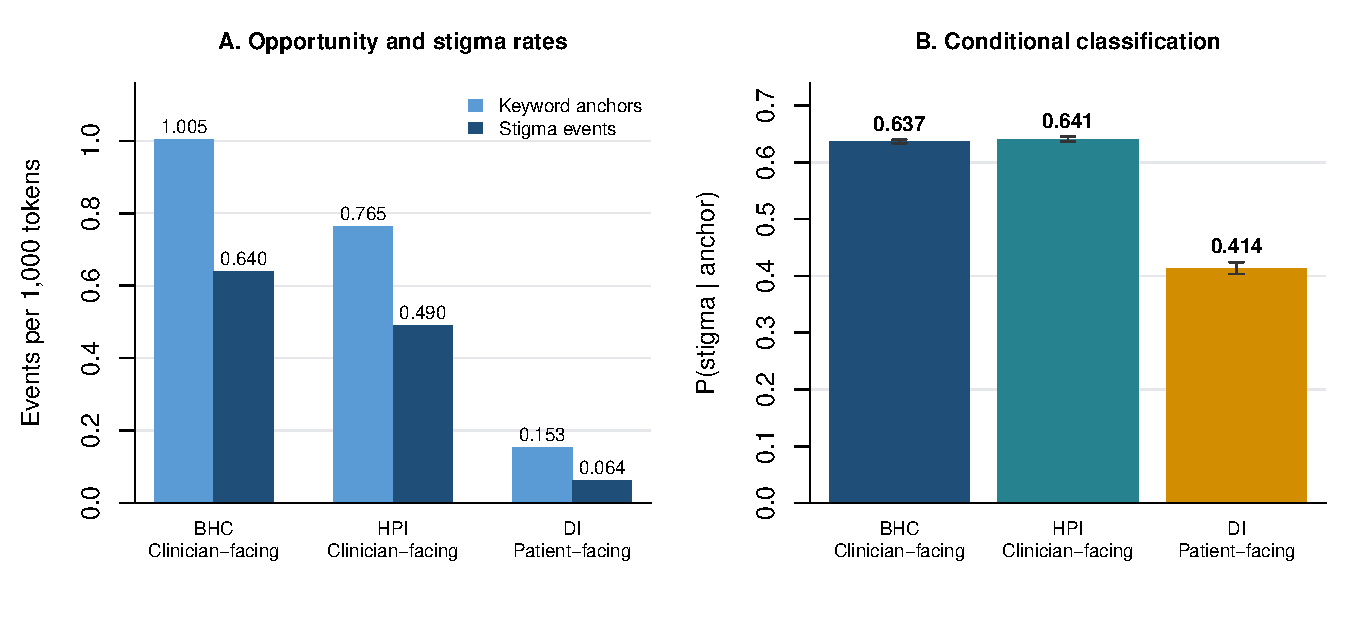
\includegraphics[width=0.98\linewidth]{figure2_decomposition.pdf}
\caption{Opportunity and conditional components across the audience boundary. Panel A pairs the successfully scored keyword-anchor and stigmatizing-language event rates for clinician-facing BHC and HPI and patient-facing DI. Panel B shows the probability that a scored anchor was stigmatizing, with descriptive candidate-level 95\% Wilson intervals based on 100,475 BHC, 45,529 HPI, and 8,613 DI candidates. Of 89 relocation failures excluded from this calculation, 72 occurred in BHC, 13 in HPI, and 4 in DI. Paired GEE, rather than these intervals, supplies inference for section contrasts. BHC, Brief Hospital Course; HPI, History of Present Illness; DI, Discharge Instructions.}
\visiblealt{Two-panel bar chart. Panel A contains paired anchor-rate and stigma-rate bars for each section, with both measures descending from BHC to HPI to DI. Panel B groups BHC and HPI at similar conditional probabilities near 0.64, while DI is lower at 0.41; narrow error bars show descriptive candidate-level 95 percent Wilson intervals.}
\label{fig:decomposition}
\end{figure}

Because whole-note rates are token-weighted averages, unequal section lengths affect the aggregate even when section-specific rates remain fixed. BHC supplied 64.0\% of combined BHC-DI tokens in the paired corpus. At the observed section rates, that aggregate mix yielded 0.433 stigmatizing-language events per 1,000 tokens. Equal BHC and DI token weights yielded 0.352, making the observed-mix value 23.0\% higher. Across individual notes, the median BHC share of BHC-plus-DI tokens was 67.6\% (interquartile range, 51.3\%-77.5\%; Supplementary Table S14).

Anchor-family classification also differed by section (Supplementary Tables S12--S13). After direct standardization to a pooled broad-family distribution, the BHC-DI conditional ratio decreased from 1.54 to 1.48 and the HPI-DI ratio from 1.55 to 1.44. Broad-family composition accounted for 6.0\% of the HPI-DI conditional probability difference and slightly masked the BHC-DI difference; most of each difference remained within the three families.

\subsection{Patient-facing DI and patient-group results}

Across all paired notes, patient-facing DI contained 3,565 stigmatizing-language events in 56,123,304 tokens. Exactly 3,003 of 259,207 notes contained at least one DI event, or 1.16\% (about 1 in 86). Repeated events in one DI increase the event rate without increasing the number of DI-positive notes. This prevalence measures occurrence in patient-facing text; patient responses were unavailable.

Absolute DI rates varied across disease cohorts (Table~\ref{tab:groups}; Figure~\ref{fig:disease}). Relative to the overall DI rate of 0.064, the DI rate for serious mental illness was 3.7 times higher (0.237; 479 events in 11,583 notes). Sickle cell disease had a rate 4.1 times overall (0.261), but this estimate came from 17 events in 419 notes and its interaction had a wide 95\% CI of 0.188-0.817. The substance use disorder DI rate was 2.5 times overall (0.158; 744 events). DI rates were 0.105 for chronic pain, 0.097 for HIV, 0.084 for end-stage renal disease, 0.067 for diabetes, and 0.040 for obesity. These values are crude rates among notes in each cohort; the interaction estimates compare the adjusted relative BHC-DI gap for cohort presence versus absence.

Absolute rates and adjusted interactions gave different rankings. Obesity widened the adjusted BHC-DI gap (RR, 1.376; 95\% CI, 1.189-1.592), yet its BHC rate of 0.598 was below the overall BHC rate of 0.640 and its DI rate of 0.040 was the lowest among the eight cohorts. Serious mental illness and sickle cell disease had narrower adjusted relative gaps while their absolute DI rates were the two highest. HIV and diabetes widened the adjusted relative gap, but their DI rates remained near the overall DI rate.

\begin{table*}[!t]
\caption{Disease-cohort absolute section rates and modification of the BHC-DI rate ratio}
\label{tab:groups}
\centering
\scriptsize
\resizebox{0.96\linewidth}{!}{%
\begin{tabular}{@{}lrrrrrrrll@{}}
\toprule
Disease cohort & Notes & BHC events & BHC rate & BHC/overall & DI events & DI rate & DI/overall & Interaction RR (95\% CI) & BH $q$ \\
\midrule
Serious mental illness & 11,583 & 10,571 & 1.872 & 2.93 & 479 & 0.237 & 3.7 & 0.725 (0.632-0.832) & $1.95\times10^{-5}$ \\
Sickle cell disease & 419 & 201 & 1.180 & 1.84 & 17 & 0.261 & 4.1 & 0.392 (0.188-0.817) & 0.025 \\
Substance use disorder & 24,425 & 15,799 & 1.340 & 2.09 & 744 & 0.158 & 2.5 & 0.910 (0.808-1.025) & 0.161 \\
Chronic pain & 14,751 & 6,118 & 0.887 & 1.39 & 291 & 0.105 & 1.6 & 0.986 (0.828-1.175) & 0.876 \\
HIV & 4,809 & 2,393 & 1.120 & 1.75 & 86 & 0.097 & 1.5 & 1.470 (1.053-2.053) & 0.038 \\
End-stage renal disease & 9,863 & 3,324 & 0.680 & 1.06 & 155 & 0.084 & 1.3 & 0.936 (0.770-1.139) & 0.582 \\
Diabetes & 71,318 & 20,576 & 0.657 & 1.03 & 1,008 & 0.067 & 1.0 & 1.275 (1.155-1.408) & $1.26\times10^{-5}$ \\
Obesity & 27,603 & 6,610 & 0.598 & 0.93 & 277 & 0.040 & 0.6 & 1.376 (1.189-1.592) & $4.87\times10^{-5}$ \\
\bottomrule
\end{tabular}}
\begin{tablenotes}
\item Rates are crude stigmatizing-language events per 1,000 tokens among notes in each disease cohort. BHC/overall and DI/overall divide the displayed cohort rates by the rounded all-note BHC rate of 0.640 or DI rate of 0.064. The covariate-adjusted interaction RR instead compares the BHC-DI RR for notes with versus without the condition; values greater than 1 indicate a wider relative section gap for the cohort. These columns therefore report related but distinct comparisons. BHC, Brief Hospital Course; DI, Discharge Instructions; BH, Benjamini-Hochberg.
\end{tablenotes}
\end{table*}

\begin{figure}[!t]
\centering
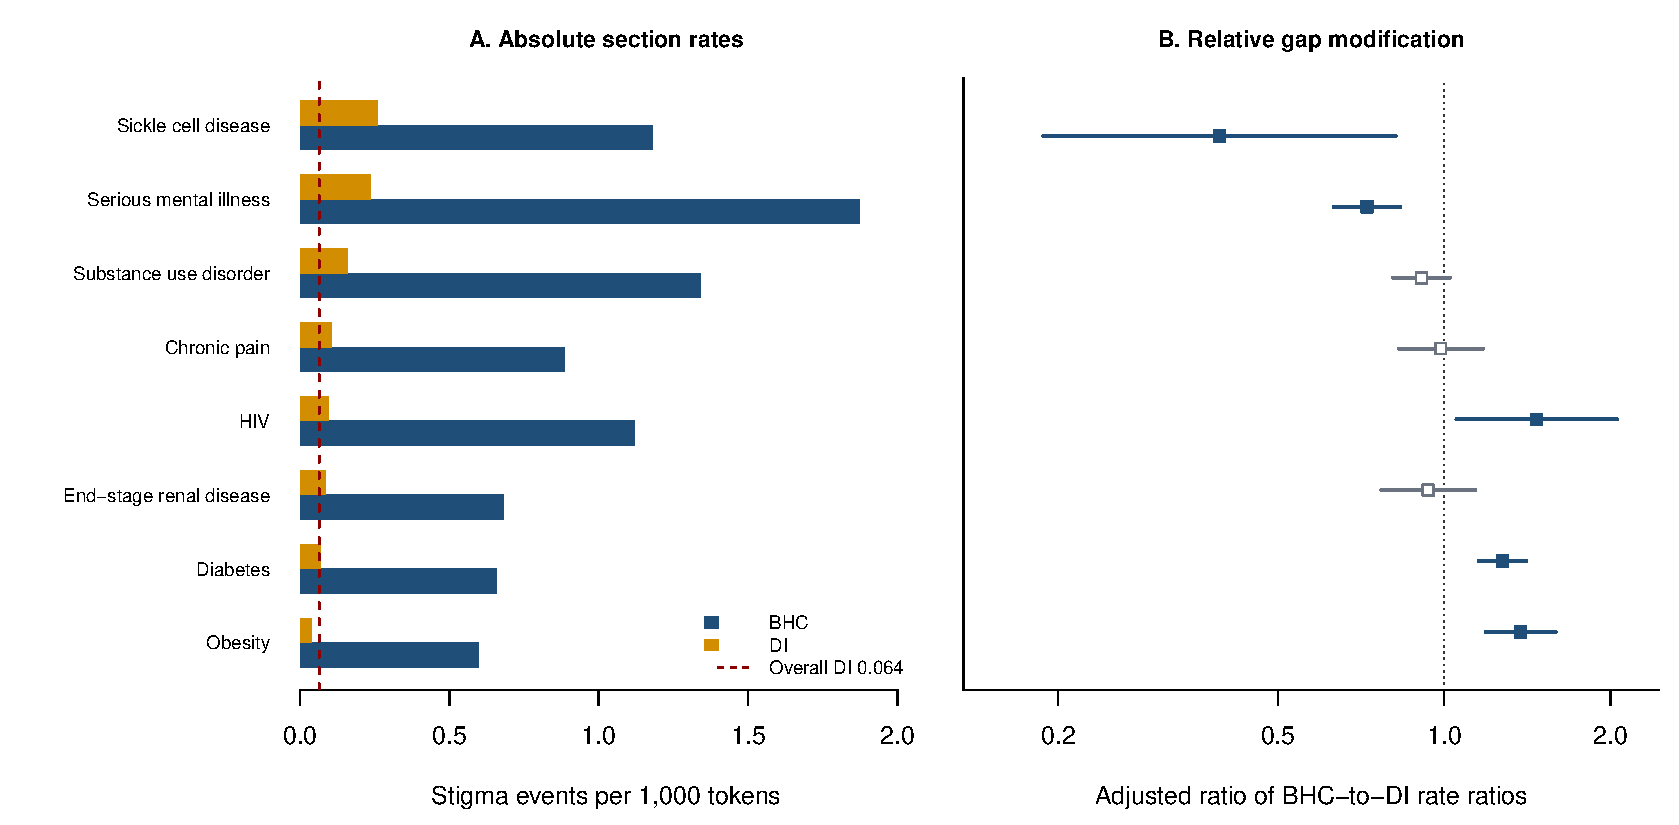
\includegraphics[width=0.99\linewidth]{figure4_disease.pdf}
\caption{Absolute and relative disease-cohort results across clinician-facing BHC and patient-facing DI. Panel A shows crude BHC and DI rates among notes in each cohort, with the all-note DI rate of 0.064 as a dashed reference. Panel B shows adjusted interaction RRs comparing the BHC-DI rate ratio for notes with versus without each condition; horizontal lines are 95\% CIs and filled squares met the Benjamini-Hochberg threshold. BHC, Brief Hospital Course; DI, Discharge Instructions.}
\visiblealt{Two-panel plot ordered by absolute DI rate. The absolute-rate panel places serious mental illness and sickle cell disease above the all-note DI reference, whereas obesity has the lowest DI rate. The interaction panel shows narrower relative gaps for the first two cohorts and a wider gap for obesity.}
\label{fig:disease}
\end{figure}

Identity results were secondary (Supplementary Table S5 and Supplementary Figure S1). Age was the only identity interaction that met the false discovery threshold in the primary log-linear model (RR per year, 0.989; 95\% CI, 0.986-0.992; $q=1.90\times10^{-14}$). Crude BHC-DI RRs decreased across age bands from 13.83 at 18--39 years to 11.94 at 40--64, 9.74 at 65--79, and 6.14 at 80 or older (Supplementary Table S15). BHC rates declined from 0.936 to 0.506 through age 65--79 before rising to 0.608 at age 80 or older; DI rates were 0.068, 0.056, 0.052, and 0.099. A restricted cubic spline diagnostic rejected a log-linear age-gap relation (joint Wald $\chi^2_2=42.16$, $P=6.99\times10^{-10}$). Relative to the gap at the mean age of 61.8 years, the adjusted spline-implied gap was 0.72 (95\% CI, 0.67-0.77) at age 80 (Supplementary Figure S2).

Several index groups had elevated crude rates even when their adjusted interactions were null. Among notes documenting Medicaid patients, the BHC rate was 0.934, 1.46 times the all-note BHC rate, and the DI rate was 0.082, 1.28 times the all-note DI rate. Among notes documenting Black patients, the corresponding rates were 0.868 (1.36 times all-note BHC) and 0.078 (1.22 times all-note DI). The adjusted Medicaid versus non-Medicaid and Black versus White interactions did not differ from 1 after false discovery correction. The descriptive comparisons use each index group versus the all-note rate; the adjusted interactions use the named reference group.

\subsection{Classifier performance and sensitivity analyses}

The fine-tuned sentence-window GatorTron classifier achieved validation macro-F1 of 0.9294 and accuracy of 0.9361; test macro-F1 was 0.9281 and accuracy was 0.9327 (Supplementary Table S1). These held-out metrics assess candidate-level binary classification but do not establish section-specific calibration.

Word10 yielded higher test macro-F1 and accuracy (0.9429 and 0.9465) than the sentence-window classifier (0.9281 and 0.9327) but remained a context-window sensitivity.

The Word10 model produced adjusted RRs of 8.26 (95\% CI, 8.01-8.51) for BHC versus DI and 7.29 (95\% CI, 7.01-7.58) for HPI versus DI. Unfiltered keyword-anchor RRs were 5.89 (95\% CI, 5.76-6.02) and 4.79 (95\% CI, 4.67-4.91), respectively. Across 10 sentence-window encoders with test accuracy above 0.90, the BHC to DI RR ranged from 8.09 to 8.79.

All sensitivity estimates retained DI as the reference and section tokens as the denominator. Contextual classification changed the magnitude of the contrasts relative to unfiltered anchors, while the direction remained consistent across context windows and qualifying encoders.

\FloatBarrier
\section{Discussion}

\subsection{Principal findings}

Stigmatizing language varied sharply across the audience boundary within the same discharge summary. The crude rate was about ten times higher in clinician-facing BHC than in patient-facing DI and 7.72 times higher in clinician-facing HPI than in DI. Most of both contrasts reflected keyword-anchor frequency, while a smaller component remained after conditioning on an anchor. The lower patient-facing rate did not mean absence: DI contained stigmatizing-language events in 3,003 notes. Disease-cohort results showed that absolute patient-facing rates and relative clinician-facing/patient-facing gaps can point in different directions.

\subsection{Interpretation}

Earlier studies established that stigma occurs in clinical records, varies across patient populations, and can be detected at scale.\cite{himmelstein2022,harrigian2023,xue2026,walker2025,scroggins2025} Our study extends this literature by centering the audience boundary within inpatient discharge summaries: patient-facing DI versus clinician-facing documentation from the same note, compared with paired token-normalized analyses.

The audience boundary changes the meaning of the observed location. In clinician-facing BHC and HPI, stigmatizing language can frame the patient for subsequent clinicians. In patient-facing DI, it appears within instructions guiding the patient's actions after discharge. The markedly lower DI rate therefore locates less stigma in patient-facing communication than in clinician-facing narrative within the same summaries. The analysis did not measure intention, clinical decisions, patient interpretation, or harm; it establishes which communication setting contained the language and where validation or review should focus.

Audience-sensitive writing is one plausible explanation for this pattern. Because DI is intended for patients to read and act on, clinicians may anticipate direct patient readership and choose wording more deliberately. DI is also typically future-oriented and instructional, emphasizing medications, follow-up, precautions, and self-care. Clinician-facing BHC and HPI instead reconstruct the encounter in a compressed third-person narrative. In doing so, they more often describe adherence, credibility, behavior, and interactions with staff, creating more occasions for evaluative wording and for situation-specific behavior to be condensed into short descriptors that can shape clinical handoff.

The decomposition supports both a narrative-opportunity explanation and a possible audience-sensitive wording explanation. The 6.55-fold BHC anchor-exposure component accounted for most of the crude clinician-facing/patient-facing difference, consistent with clinician-facing narrative having more occasions to describe patient behavior. DI also had a lower probability of stigma conditional on an anchor. This smaller conditional difference is consistent with more careful wording for a patient audience, but it does not demonstrate clinicians' intentions. Direct standardization showed that the conditional contrast persisted after equalizing the three broad anchor families: the BHC-DI ratio was 1.48 and the HPI-DI ratio was 1.44. The standardized comparison still combines exact keyword mix, contextual use, and classifier behavior; it does not isolate a causal effect of audience.

Because BHC and DI come from the same admission and summary, pairing removes between-admission differences from the audience comparison. The sections nevertheless differ in content, timing, conventional voice, and possible author. The contrast therefore shows how stigma is distributed between clinician-facing and patient-facing documentation but does not isolate audience as the cause of that distribution. HPI strengthens the pattern by providing a second clinician-facing section with a similar conditional point estimate, although no equivalence test was performed.

The token totals show why the aggregation choice matters. BHC made up 64.0\% of combined BHC-DI tokens, and the observed mix yielded a composite rate 23.0\% higher than equal token weights at fixed section rates. The per-note BHC share varied widely, with a 5th-to-95th percentile range of 26.1\% to 86.7\%. These quantities describe composition, not a causal template effect. A whole-note dashboard can therefore change because within-section language changed, document composition changed, or both.

The disease results illustrate the distinction between absolute section rates and relative-gap modification. Obesity had a wider adjusted BHC-DI gap, although both its BHC rate and its DI rate were low; serious mental illness had a narrower relative gap but a DI rate 3.7 times the all-note rate. Age provided a second example: the crude gap narrowed across age bands because the two absolute section rates followed different, nonlinear patterns, especially at older ages. Medicaid and Black index groups had crude rates above the corresponding all-note rates in both sections, while their adjusted interactions relative to non-Medicaid and White reference groups were null after false discovery correction. Reporting only interaction significance would omit those descriptive elevations, whereas treating crude elevations as adjusted identity effects would exceed the analysis.

Equity reporting needs both quantities because they use different comparisons. The interaction compares adjusted relative BHC-DI gaps between an index and reference group, whereas the crude section rate describes stigmatizing-language events per token within the index group. A null interaction can therefore coexist with elevated crude rates in both sections. Stating the denominator, index population, and reference for each estimate prevents a null relative-gap result from being read as evidence of equal absolute rates.

The DI-specific result gives a direct reason to preserve section identity. DI is patient-facing, and 3,003 notes contained at least one stigmatizing-language event there. Its lower average rate does not mean stigma is absent from patient-facing communication. Evaluating patient interpretation, trust, comprehension, or harm requires patient-level outcome data.

\subsection{Implications for informatics practice}

Stigma surveillance dashboards and documentation-equity audits should retain the clinician-facing/patient-facing distinction. A whole-note rate cannot show whether stigmatizing language occurred in clinician-facing documentation or patient-facing DI, and it blends within-section language with token composition. A practical display would report notes, tokens, stigmatizing-language events, and event rates by section, retain the whole-note rate as a secondary summary, and label absolute rates separately from interaction estimates. This design lets analysts identify both the intended audience of the text and whether an apparent change reflects documentation structure rather than language within a section.

Authoring support should also account for section audience. Generic whole-note alerts ignore differences in anchor opportunity and contextual use between clinician-facing narrative and patient-facing instructions. A section-aware tool should show the full sentence context rather than blacklist an anchor, because the same term may be stigmatizing or neutral depending on context and these patterns vary by section. Any review threshold would require section-stratified human labels before deployment.

Stigmatizing-language events occurred in DI in 1.16\% of paired notes, which sets the scale for review of patient-facing text. An alert attached to every discharge summary would be poorly targeted because most notes had no DI event. Targeted retrospective review or sampled auditing is more consistent with the observed prevalence, although prospective workflow effects were not evaluated. The high patient-facing DI rate for serious mental illness and the sparse sickle cell estimate identify priorities for qualitative validation and patient co-design, not grounds for automated judgments about clinicians or patients.

\subsection{Limitations}

This retrospective analysis reflects one deidentified academic-center corpus, whose templates and documentation practices define the study setting. The classifier covers only expressions containing 89 predefined terms and excludes open-vocabulary forms from its estimand. Training annotations came mainly from third-person clinical contexts, and section-stratified labels were unavailable, so calibration may differ between clinician-facing and patient-facing sections. Header parsing and the 50-token threshold favor summaries that follow recognizable templates. Within-note pairing holds the patient, admission, and document constant, but section authorship remains unobserved. Broad-family standardization does not control the exact keyword mix or section-specific classifier error. Administrative race and ethnicity, sex, language, and insurance fields incompletely represent social identity. Coding missing insurance as non-Medicaid and missing language as English may distort group comparisons. Age-band rates are crude, and the spline analysis is a functional-form diagnostic rather than a causal age effect. Sparse events in some cohorts, residual clinical differences, and the observational design further limit causal interpretation of section and group contrasts. DI is patient-facing, but MIMIC-IV-Note does not contain patient responses; the study therefore does not establish how patients interpreted or were affected by the language.

\section{Conclusion}

Stigmatizing language was strongly patterned by audience within discharge summaries. Rates were substantially higher in clinician-facing hospital course and history sections than in patient-facing DI, and most of the difference reflected the greater number of keyword-anchor opportunities in clinician-facing narrative. Stigmatizing-language events nevertheless occurred in patient-facing DI in 1.16\% of notes, with higher absolute DI rates in some disease cohorts. Section-specific reporting distinguishes language circulating in clinician-facing documentation from language appearing in patient-facing instructions and prevents document composition from being mistaken for a change in language. These results are limited to MIMIC-IV and do not establish a causal effect of audience, patient response, or performance beyond this corpus.

\section*{Acknowledgments}


\section*{Funding}

\textit{Author input required: insert funder names and grant numbers, or confirm that the work received no specific funding.}

\section*{Competing Interests}

\textit{Author input required: provide the author-approved competing-interests statement.}

\section*{Author Contributions (CRediT)}

\textit{Author input required: assign CRediT taxonomy roles to every named author.}

\section*{Data Availability}

MIMIC-IV-Note version 2.2 and MIMIC-IV version 2.2 are available from PhysioNet to credentialed users who complete the required training and sign the data use agreement. Patient-level text and derived row-level data remain governed by those access terms. \textit{Author input required: confirm the release scope and insert the public repository URL and archival identifier.}

\section*{Code Availability}

\textit{Author input required: confirm which analysis code, figure-generating code, machine-readable aggregate results, environment specification, and permitted model artifacts will be released; then insert the repository URL, archival identifier, and model checksum.}

\section*{Ethics Statement}

This secondary analysis used deidentified data under PhysioNet credentialing and data use terms. The MIMIC data-sharing initiative was approved by the Beth Israel Deaconess Medical Center Institutional Review Board with a waiver of informed consent. \textit{Author input required: add the authors' institutional determination, protocol number if applicable, and study-specific consent determination.}

% \begin{thebibliography}{99}

% \bibitem{link2001} Link BG, Phelan JC. Conceptualizing stigma. \textit{Annu Rev Sociol} 2001;27:363-385. doi:10.1146/annurev.soc.27.1.363.

% \bibitem{hatzenbuehler2013} Hatzenbuehler ML, Phelan JC, Link BG. Stigma as a fundamental cause of population health inequalities. \textit{Am J Public Health} 2013;103:813-821. doi:10.2105/AJPH.2012.301069.

% \bibitem{goddu2018} Goddu AP, O'Conor KJ, Lanzkron S, et al. Do words matter? Stigmatizing language and the transmission of bias in the medical record. \textit{J Gen Intern Med} 2018;33:685-691. doi:10.1007/s11606-017-4289-2.

% \bibitem{park2021} Park J, Saha S, Chee B, et al. Physician use of stigmatizing language in patient medical records. \textit{JAMA Netw Open} 2021;4:e2117052. doi:10.1001/jamanetworkopen.2021.17052.

% \bibitem{mcarthur2026} McArthur A, Ahmad A, Links AR, et al. How words discredit: a taxonomy of stigmatizing language in the electronic health record. \textit{Patient Educ Couns} 2026;147:109520. doi:10.1016/j.pec.2026.109520.

% \bibitem{himmelstein2022} Himmelstein G, Bates D, Zhou L. Examination of stigmatizing language in the electronic health record. \textit{JAMA Netw Open} 2022;5:e2144967. doi:10.1001/jamanetworkopen.2021.44967.

% \bibitem{harrigian2023} Harrigian K, Zirikly A, Chee B, et al. Characterization of stigmatizing language in medical records. In: \textit{Proceedings of the 61st Annual Meeting of the Association for Computational Linguistics, Volume 2: Short Papers}. Toronto, Canada: Association for Computational Linguistics 2023:312-329. doi:10.18653/v1/2023.acl-short.28.

% \bibitem{xue2026} Xue L, Rahman AMM, Senteio CR, et al. Automated detection of stigmatizing language in electronic health records using a multi-stage transfer learning approach. \textit{J Am Med Inform Assoc} 2026;33:283-294. doi:10.1093/jamia/ocaf193.

% \bibitem{walker2025} Walker A, Thorne A, Das S, et al. CARE-SD: classifier-based analysis for recognizing provider stigmatizing and doubt marker labels in electronic health records: model development and validation. \textit{J Am Med Inform Assoc} 2025;32:365-374. doi:10.1093/jamia/ocae310.

% \bibitem{scroggins2025} Scroggins JK, Hulchafo II, Harkins S, et al. Identifying stigmatizing and positive/preferred language in obstetric clinical notes using natural language processing. \textit{J Am Med Inform Assoc} 2025;32:308-317. doi:10.1093/jamia/ocae290.

% \bibitem{mimicnote2023} [dataset] Johnson A, Pollard T, Horng S, et al. MIMIC-IV-Note: deidentified free-text clinical notes. PhysioNet 2023. Version 2.2. doi:10.13026/1n74-ne17.

% \bibitem{mimiciv2023} [dataset] Johnson A, Bulgarelli L, Pollard T, et al. MIMIC-IV. PhysioNet 2023. Version 2.2. doi:10.13026/6mm1-ek67.

% \bibitem{yang2022} Yang X, Chen A, PourNejatian N, et al. A large language model for electronic health records. \textit{NPJ Digit Med} 2022;5:194. doi:10.1038/s41746-022-00742-2.

% \bibitem{zeger1986} Zeger SL, Liang KY. Longitudinal data analysis for discrete and continuous outcomes. \textit{Biometrics} 1986;42:121-130. PMID:3719049.

% \bibitem{charlson1987} Charlson ME, Pompei P, Ales KL, et al. A new method of classifying prognostic comorbidity in longitudinal studies: development and validation. \textit{J Chronic Dis} 1987;40:373-383. doi:10.1016/0021-9681(87)90171-8.

% \bibitem{quan2005} Quan H, Sundararajan V, Halfon P, et al. Coding algorithms for defining comorbidities in ICD-9-CM and ICD-10 administrative data. \textit{Med Care} 2005;43:1130-1139. doi:10.1097/01.mlr.0000182534.19832.83.

% \bibitem{benjamini1995} Benjamini Y, Hochberg Y. Controlling the false discovery rate: a practical and powerful approach to multiple testing. \textit{J R Stat Soc Series B Stat Methodol} 1995;57:289-300. doi:10.1111/j.2517-6161.1995.tb02031.x.

% @article{li2026readability,
%   author  = {Li, Fuchen and Taylor, Casey Overby and Zirikly, Ayah},
%   title   = {A Multi-Metric Evaluation of Readability in Psychiatric Discharge Summaries},
%   journal = {BioData Mining},
%   year    = {2026},
%   volume  = {19},
%   number  = {1},
%   pages   = {27},
%   doi     = {10.1186/s13040-026-00528-2},
%   url     = {https://doi.org/10.1186/s13040-026-00528-2}
% }

% @inproceedings{xu2024dischargeme,
%   author    = {Xu, Justin and Chen, Zhihong and Johnston, Andrew and
%                Blankemeier, Louis and Varma, Maya and Hom, Jason and
%                Collins, William J. and Modi, Ankit and Lloyd, Robert and
%                Hopkins, Benjamin and Langlotz, Curtis and
%                Delbrouck, Jean-Benoit},
%   title     = {Overview of the First Shared Task on Clinical Text Generation:
%                {RRG}24 and ``Discharge Me!''},
%   booktitle = {Proceedings of the 23rd Workshop on Biomedical Natural Language Processing},
%   year      = {2024},
%   month     = aug,
%   address   = {Bangkok, Thailand},
%   publisher = {Association for Computational Linguistics},
%   doi       = {10.18653/v1/2024.bionlp-1.7},
%   url       = {https://aclanthology.org/2024.bionlp-1.7}
% }

% @article{goddu2018,
%   author  = {Goddu, Anna P. and O'Conor, Katie J. and Lanzkron, Sophie and
%              Saheed, Mustapha O. and Saha, Somnath and Beach, Mary Catherine},
%   title   = {Do Words Matter? Stigmatizing Language and the Transmission of Bias in the Medical Record},
%   journal = {Journal of General Internal Medicine},
%   year    = {2018},
%   volume  = {33},
%   number  = {5},
%   pages   = {685--691},
%   doi     = {10.1007/s11606-017-4289-2},
%   url     = {https://doi.org/10.1007/s11606-017-4289-2}
% }

% @article{leveille2020notes,
%   author  = {Leveille, Suzanne G. and Fitzgerald, Patricia and Harcourt, Kendall and
%              Dong, Zhiyong and Bell, Sigall and O'Neill, Steve and
%              DesRoches, Catherine and Fernandez, Leonor and Jackson, Sara L. and
%              Klein, Jared W. and Stametz, Rebecca and Delbanco, Tom and Walker, Jan},
%   title   = {Patients Evaluate Visit Notes Written by Their Clinicians:
%              A Mixed Methods Investigation},
%   journal = {Journal of General Internal Medicine},
%   year    = {2020},
%   volume  = {35},
%   number  = {12},
%   pages   = {3510--3516},
%   doi     = {10.1007/s11606-020-06014-7},
%   url     = {https://doi.org/10.1007/s11606-020-06014-7}
% }

% \end{thebibliography}

\bibliographystyle{unsrt}

\bibliography{references}
\end{document}
